\documentclass[11pt]{article}
\usepackage[utf8]{inputenc}
\usepackage[british]{babel}
\usepackage{csquotes}
\usepackage[margin=1in]{geometry}
\usepackage{microtype}
\usepackage{amsmath}
\usepackage{amssymb}
\usepackage{amsthm}
%\usepackage[style=S]{thmbox}
\usepackage{cmll}
\usepackage{libertine}
\usepackage[scale=0.8]{sourcecodepro}
\usepackage{stmaryrd}
\usepackage{mathpartir}
\usepackage{ebproof}
\usepackage[
    style=alphabetic
]{biblatex}
\addbibresource{report.bib}
%\DeclareLabelalphaTemplate{
%    \labelelement{
%        \field[ifnames=1,strwidth=10]{labelname}
%        \field[ifnames=2-,strwidth=1]{labelname}
%    }
%    \labelelement{
%        \field[strwidth=2,strside=right]{year}
%    }
%}
\usepackage{xcolor}
\definecolor{linkcolor}{HTML}{DD00BB}
\usepackage[
    pdfauthor={Naïm Favier},
    bookmarksopen=true,
    colorlinks=true,
    allcolors=linkcolor
]{hyperref}
\usepackage{cleveref}
\usepackage[sc]{titlesec}

\author{Naïm Favier}

\setlength{\parskip}{0.5em}
\renewcommand\labelitemi{$\circ$}

\newtheorem{definition}{Definition}[section]
\newtheorem{theorem}{Theorem}[section]
\newtheorem{lemma}[theorem]{Lemma}
\newtheorem{corollary}{Corollary}[theorem]

\newcommand\LL{\textsf{LL}}
\newcommand\MALL{\textsf{MALL}}
\newcommand\0{\textbf{0}}
\newcommand\1{\textbf{1}}
\newcommand\LLfoc{{\LL_\text{foc}}}
\newcommand\LLFoc{{\LL_\text{Foc}}}
\newcommand\size[1]{{\lvert #1 \rvert}}
\newcommand\sem[1]{{\llbracket #1 \rrbracket}}
\newcommand\biperp{{\perp\perp}}
\newcommand\triperp{{\perp\perp\perp}}
\newcommand\Foc{\textup{Foc}}

\usepackage{titling}
\title{\huge\sc Phase semantics of linear logic applied to the focalisation property}
\author{Naïm Favier --- ENS Paris}
\date{1st April -- 31st August 2021}
\renewcommand\maketitlehookd{
    \centering
    M1 research internship supervised by: Alexis Saurin --- PPS pole --- IRIF

    \vspace{15px}
    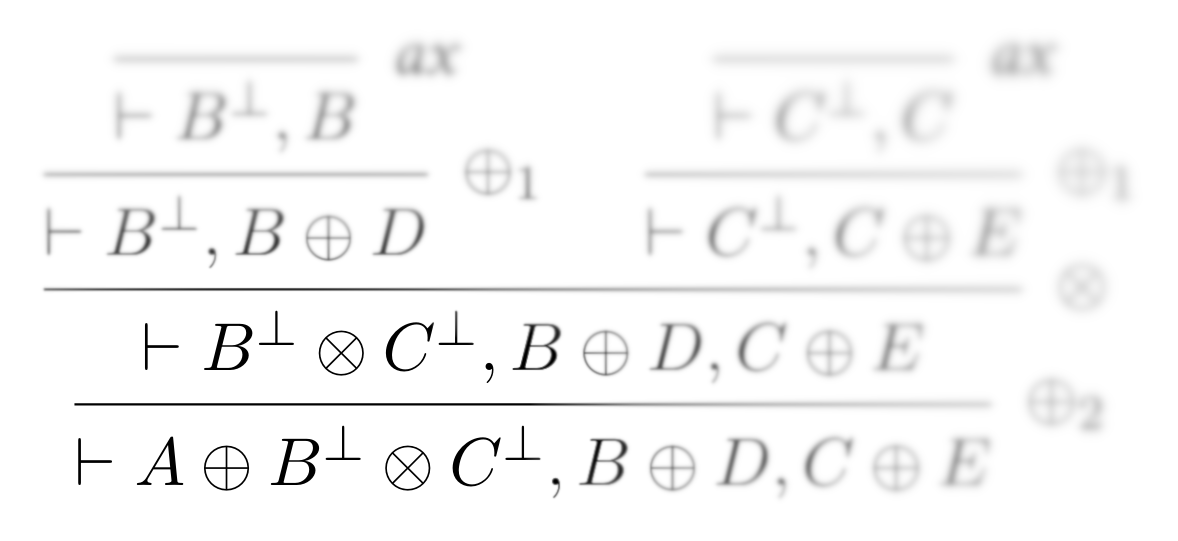
\includegraphics[width=300px]{focus}

%$$
%\scalebox{1.5}{
%\begin{prooftree}
%    \infer0[\textit{ax}]{\vdash B^\perp, B}
%    \infer1[$\oplus_1$]{\vdash B^\perp, B \oplus D}
%    \infer0[\textit{ax}]{\vdash C^\perp, C}
%    \infer1[$\oplus_1$]{\vdash C^\perp, C \oplus E}
%    \infer2[$\otimes$]{\vdash B^\perp \otimes C^\perp, B \oplus D, C \oplus E}
%    \infer1[$\oplus_2$]{\vdash A \oplus B^\perp \otimes C^\perp, B \oplus D, C \oplus E}
%\end{prooftree}
%}
%$$
}

\usepackage{graphicx}

\begin{document}

\maketitle

\section{Introduction}

{\sc Linear logic}, introduced by Jean-Yves Girard in the late 1980s~\cite{ll}, is a logic that stems from
the continuation of the path from classical to intuitionistic logic,
and has proven to have many fruitful applications, from functional programming to quantum mechanics.
The most common interpretation of linear logic is in term of \emph{resources}: where classical logic allows one to use
each hypothesis as many times as one wants (including not at all) by using the weakening and contraction rules,
linear logic gets rid of these rules, hence requiring that each premise be used \emph{exactly} once, as in e.g. a chemical reaction.

During this internship, I have been investigating the phase semantics of linear logic, a simple semantics
of \emph{provability}, and trying to extract information on \emph{proofs} from such semantics, in particular in relationship
to the focalisation property which allows a proof search procedure to narrow down its search space in certain situations.

We will start with a basic review of linear logic in \cref{sec:ll}, then we'll introduce phase semantics and their main
completeness results in \cref{sec:phase_semantics}, and finally we'll explore the application of phase semantics
to the focalisation property in \cref{sec:focalisation}.

\section{\label{sec:ll}Linear logic}

Linear logic arises from the removal of the weakening and contraction rules from classical logic.
This prohibition splits the usual connectives of classical logic into
\emph{multiplicative} and \emph{additive} variants:
\begin{center}
    \begin{tabular}{c|c|c}
        classical & $\LL$ (multiplicative) & $\LL$ (additive) \\
        \hline
        $\land$ & $\otimes$ & $\with$ \\
        $\lor$ & $\parr$ & $\oplus$ \\
        $\top$ & $1$ & $\top$ \\
        $\bot$ & $\bot$ & $0$
    \end{tabular}
\end{center}
where $\otimes$, $\oplus$, $\with$ and $\parr$ are associative and commutative, and $1$, $0$, $\top$ and $\bot$ are
their respective units (and nullary versions).

In order to keep the expressive power of classical logic, we reintroduce weakening and contraction in a \emph{controlled}
manner under the connectives $\oc$ and $\wn$. In the resource interpretation, $\oc A$ can be understood as an infinite
source of $A$ that can be used or discarded as one wishes.

There is an elegant symmetry in linear logic, embodied by the involutive \emph{linear negation} $\cdot^\perp$,
which is defined inductively on formulas using De Morgan laws:

\begin{align*}
    (A \otimes B)^\perp &= A^\perp \parr B^\perp & (A \parr B)^\perp &= A^\perp \otimes B^\perp \\
    (A \oplus B)^\perp &= A^\perp \with B^\perp & (A \with B)^\perp &= A^\perp \oplus B^\perp \\
    1^\perp &= \bot & \bot^\perp &= 1 \\
    0^\perp &= \top & \top^\perp &= 0 \\
    (\oc A)^\perp &= \wn A & (\wn A)^\perp &= \oc A \\
    (X)^\perp &= X^\perp & (X^\perp)^\perp &= X
\end{align*}

We now present the one-sided sequent calculus for linear logic, $\LL$. A context (noted $\Gamma$, $\Delta$, \dots)
is a multiset of formulas, and a sequent has the general form $\Gamma \vdash \Delta$. However,
such a sequent is equivalent to $\vdash \Gamma^\perp, \Delta$, so it is enough to consider sequents with only
formulas on the right.

The inference rules for $\LL$ are as follows:
\begin{gather*}
    \begin{prooftree}
        \infer0[\textit{ax}]{\vdash A, A^\perp}
    \end{prooftree}
    \qquad
    \begin{prooftree}
        \hypo{\vdash \Gamma, A}
        \hypo{\vdash A^\perp, \Delta}
        \infer2[\textit{cut}]{\vdash \Gamma, \Delta}
    \end{prooftree}
    \\
    \begin{prooftree}
        \hypo{\vdash \Gamma, A, B}
        \infer1[$\parr$]{\vdash \Gamma, A \parr B}
    \end{prooftree}
    \qquad
    \begin{prooftree}
        \hypo{\vdash \Gamma}
        \infer1[$\bot$]{\vdash \Gamma, \bot}
    \end{prooftree}
    \\
    \begin{prooftree}
        \hypo{\vdash \Gamma, A}
        \hypo{\vdash \Delta, B}
        \infer2[$\otimes$]{\vdash \Gamma, \Delta, A \otimes B}
    \end{prooftree}
    \qquad
    \begin{prooftree}
        \infer0[$1$]{\vdash 1}
    \end{prooftree}
    \\
    \begin{prooftree}
        \hypo{\vdash \Gamma, A}
        \hypo{\vdash \Gamma, B}
        \infer2[$\with$]{\vdash \Gamma, A \with B}
    \end{prooftree}
    \qquad
    \begin{prooftree}
        \infer0[$\top$]{\vdash \Gamma, \top}
    \end{prooftree}
    \\
    \begin{prooftree}
        \hypo{\vdash \Gamma, A}
        \infer1[$\oplus_1$]{\vdash \Gamma, A \oplus B}
    \end{prooftree}
    \qquad
    \begin{prooftree}
        \hypo{\vdash \Gamma, B}
        \infer1[$\oplus_2$]{\vdash \Gamma, A \oplus B}
    \end{prooftree}
    \\
    \begin{prooftree}
        \hypo{\vdash \wn\Gamma, A}
        \infer1[$\oc$]{\vdash \wn\Gamma, \oc A}
    \end{prooftree}
    \qquad
    \begin{prooftree}
        \hypo{\vdash \Gamma, A}
        \infer1[$\wn d$]{\vdash \Gamma, \wn A}
    \end{prooftree}
    \qquad
    \begin{prooftree}
        \hypo{\vdash \Gamma}
        \infer1[$\wn w$]{\vdash \Gamma, \wn A}
    \end{prooftree}
    \qquad
    \begin{prooftree}
        \hypo{\vdash \Gamma, \wn A, \wn A}
        \infer1[$\wn c$]{\vdash \Gamma, \wn A}
    \end{prooftree}
\end{gather*}

\emph{Linear implication}, noted $A \multimap B$, is defined as $A^\perp \parr B$.

Remarkably, $\otimes$ and $\oplus$ distribute over each other; dually,
$\parr$ and $\with$ distribute each other; finally, we have $\oc (A \with B) \equiv \oc A \otimes \oc B$.

\section{\label{sec:phase_semantics}Phase semantics}

Linear logic has two main semantics: coherence spaces, which is a semantics of \emph{proofs}, and phase semantics,
a simpler semantics of \emph{provability} which we will focus on.

\begin{definition}
    A \textbf{phase space} consists of a commutative monoid $M$ of \emph{phases} (written multiplicatively)
    and a subset $\bot \subseteq M$ of \emph{antiphases}.
\end{definition}

The linear negation of a set of phases $X \subseteq M$ is defined as $X^\perp = \{m \in M \mid \forall x \in X, m \cdot x \in \bot\}$.
For any $X, Y \subseteq M$, we have the following easy results:
\begin{itemize}
    \item $X \subseteq X^\biperp$
    \item $X \subseteq Y \implies Y^\perp \subseteq X^\perp$
    \item $X^\perp = X^\triperp$
    \item $(X \cup Y)^\perp = X^\perp \cap Y^\perp$
\end{itemize}

A \emph{fact} is a set of phases $X$ such that $X = X^\biperp$. Equivalently, a fact is a set of the form $Y^\perp$
for $Y \subseteq M$.

We define the following operators and constants on $\mathcal P(M)$:
\begin{align*}
    X \otimes Y &= (X \cdot Y)^\biperp & X \parr Y &= (X^\perp \cdot Y^\perp)^\perp \\
    X \oplus Y &= (X \cup Y)^\biperp & X \with Y &= X \cap Y \\
    \1 &= \bot^\perp \\
    \0 &= \top^\perp & \top &= M \\
    I &= \{m \in M \mid\, m\cdot m = m\}\text{ (the set of \textit{idempotents})} \\
    \oc X &= (X \cap \1 \cap I)^\biperp & \wn X &= (X^\perp \cap \1 \cap I)^\perp
\end{align*}

Let $\Phi$ be an $n$-ary monotonous operator on $\mathcal P(M)$. $\Phi$ is
\begin{itemize}
    \item[$-$] \textbf{negative} if it maps facts to facts, i.e. $\Phi(X_1^\biperp, \dots, X_n^\biperp)^\biperp = \Phi(X_1^\biperp, \dots, X_n^\biperp)$;
    \item[$+$] \textbf{positive} if it verifies $\Phi(X_1^\biperp, \dots, X_n^\biperp) \subseteq \Phi(X_1, \dots, X_n)^\biperp$.
\end{itemize}
In the nullary case, every set of phases is positive and the negative sets of phases are exactly facts.

\begin{definition}
    A \textbf{phase model} is a phase space $(M, \bot)$ together with a fact $\sem{X}$ for every atomic
    formula $X$. The interpretation $\sem{A}$ of a formula $A$ is defined by induction using the operators above,
    and the interpretation of a context $\Gamma = A_1, \ldots, A_n$ is defined as $\sem{\Gamma} = \sem{A_1} \parr \dots \parr \sem{A_n}$.
    Clearly $\sem{A}$, $\sem{\Gamma}$ are facts.
\end{definition}

A formula is said to be \emph{valid} in a given phase model if $1 \in \sem{A}$. More generally, a sequent
$\vdash \Gamma$ is valid if $1 \in \sem{\Gamma}$.

\begin{theorem}[Soundness]
    If a sequent $\vdash \Gamma$ is provable in $\LL$, then it is valid in every phase model.
\end{theorem}
\begin{proof}
    By induction on a proof of $\vdash \Gamma$. See for example \cite[theorem 1]{okada}.
\end{proof}

\begin{theorem}[Completeness]
    If a sequent $\vdash \Gamma$ is valid in every phase model, then it is provable in $\LL$.
\end{theorem}

This statement can actually be made stronger:
\begin{theorem}[Cut-free completeness]
    If a sequent $\vdash \Gamma$ is valid in every phase model, then it has a cut-free proof in $\LL$.
\end{theorem}
\begin{proof}
    By induction on $\Gamma$ (considered as a single formula). See \cite[theorem 3]{okada}.
\end{proof}

Combining the cut-free completeness theorem with the soundness theorem, we get:
\begin{theorem}[Cut elimination]
    If a sequent $\vdash \Gamma$ is provable in $\LL$, then it has a cut-free proof.
\end{theorem}

\section{\label{sec:focalisation}The focalisation property}

Proof search is the problem of finding a proof of a given sequent. It can be expressed recursively, starting
from a root sequent and working its way up towards the leaves (e.g. axiom rules). At each step, the procedure
must choose a formula in the current sequent, a rule to obtain that formula, and possibly the prerequisites for
that rule. In fact, we can observe that the only connectives whose introduction rule requires making a choice are
$\otimes$ and $\oplus$: the $\otimes$ rule requires choosing a way to split the context into two, while the $\oplus$
connective requires choosing between the $\oplus_1$ and $\oplus_2$ rules.

This suggests another partition of the connectives into two \emph{polarities}, the \emph{positive} connectives
($\otimes$, $\oplus$, $1$, $0$, $\oc$) and the \emph{negative} connectives ($\parr$, $\with$, $\bot$, $\top$, $\wn$).
Notice that the remarkable distributivities of \cref{sec:ll} only occur between connectives of the same polarities,
and that linear negation flips the polarity of a formula (which is defined as the polarity of its main connective).

A crucial property of the proof theory of linear logic is the \emph{focalisation} (or \emph{focusing}) property,
discovered by Jean-Marc Andreoli~\cite{andreoli}, which allows the search space to be reduced by "focusing" on certain
connectives.

The property has two sides:
\begin{itemize}
    \item[$-$] negative connectives are \emph{reversible}: in a sequent with negative formulas,
    we can always start by applying the introduction rules for the negative connectives without risk;
    \item[$+$] positive connectives can be grouped into a maximal cluster and handled all at once.
    For example, given the formula $A \oplus (B \otimes C)$, if we decide to decompose it using the $\oplus_2$ rule,
    then we can immediately decompose $B \otimes C$ using the $\otimes$ rule without needing to backtrack.
\end{itemize}

The focalisation property already has several syntactic proofs \cite{andreoli} \cite{saurin} \cite{laurent}; the main
contribution of this internship is a \emph{semantic} proof of the completeness of focused proofs
using phase semantics.

Laurent's proof~\cite{laurent} proceeds in two steps: it first embeds proofs of $\LL$ into proofs of $\LLfoc$, a
restricted variant of $\LL$ that enforces a \emph{weak} focalisation property (the core of the proof),
then it embeds cut-free proofs of $\LLfoc$ into proofs of $\LLFoc$, an even more restricted system that enforces
the full focalisation property.

We prove that phase semantics are complete with respect to the cut-free $\LLfoc$ system. Combined with the soundness theorem
and \cite[proposition 1]{laurent}, we get that every sequent that is provable in $\LL$ has a weakly focalised proof.

In the following, let $\vdash \Gamma; \Pi$ (where $\Pi$ is either empty or a single positive formula) denote a sequent
of $\LLfoc$ \emph{without the cut rules}.
To simplify the notation, we let $\vdash \Gamma; N$ mean $\vdash \Gamma, N;$ when $N$ is a negative formula.

\begin{definition}
We define the \textbf{focalised syntactic phase model} as $(M, \bot)$ where $M$ is the
free commutative monoid over formulas of $\LL$ with $\wn A$ and $\wn A, \wn A$ identified,
$\bot = \{\Gamma \in M \mid\,\vdash \Gamma;\}$, and
$\sem{X} = \{X^\perp\}^\biperp$ for positive atoms $X$. We have $\Gamma \cdot \Delta = \Gamma, \Delta$ and $1 = \emptyset$.
\end{definition}

Let $\Foc(A) = {\{\Gamma \in M \mid\, \vdash \Gamma; A\}}$.
Clearly $\Foc(A) \subseteq \{A\}^\perp$ by the \textit{foc} rule, and in particular
$\Foc(N) = \{N\}^\perp$ for $N$ negative.

Note that provability is compatible with our identification of $\wn A$ and $\wn A, \wn A$ thanks to the $\wn w$ and $\wn c$ rules,
so that $\bot$ and $\Foc$ are well-defined. Also note that $I = \{\wn \Gamma\mid\,\Gamma\in M\} \subseteq \1$ because of the
$\wn w$ rule, so that $\sem{\oc A} = (\sem{A} \cap I)^\biperp$.

We use the decomposition of exponential connectives alluded to in \cite[section 4.1]{laurent}: \begin{align*}
    \oc A &= \shpos\sharp A & \wn A &= \shneg\flat A
\end{align*}
where $\shpos, \flat$ are positive and $\sharp, \shneg$ are negative.
In fact, we only need to consider formulas of the forms $A$ and $\sharp A$, where $A$ is a formula of $\LL$.
Let us extend our definitions to this connective
with $\sem{\sharp A} = \sem{\oc A}$ and $\Foc(\sharp A) = \{A\}^\perp \cap I$.

For a formula $A$, let $\size{A}$ denote the number of main negative subformulas in $A$
(where $\sharp B$ is the main negative subformula in $\oc B$).

Let $\Psi_A$ be an $\size{A}$-ary positive operator on $\mathcal P(M)$ defined by induction as follows:
\begin{itemize}
    \item $\Psi_N(N_1) = N_1$ if $N$ is negative
    \item $\Psi_X() = \{X^\perp\}$
    \item $\Psi_{B \otimes C}(B_1, \dots, B_\size{B}, C_1, \dots, C_\size{C}) = \Psi_B(B_1, \dots, B_\size{B}) \cdot \Psi_C(C_1, \dots, C_\size{C})$
    \item $\Psi_{B \oplus C}(B_1, \dots, B_\size{B}, C_1, \dots, C_\size{C}) = \Psi_B(B_1, \dots, B_\size{B}) \cup \Psi_C(C_1, \dots, C_\size{C})$
    \item $\Psi_1() = \{\emptyset\}$
    \item $\Psi_0() = \emptyset$
    \item $\Psi_{\oc B}(B_1) = B_1$
\end{itemize}

\begin{lemma}
    \label{positivity}
    For any formula A with main negative subformulas $A_1, \dots, A_\size{A}$,
    $$\sem{A} \subseteq \Psi_A(\sem{A_1}, \dots, \sem{A_\size{A}})^\biperp$$
\end{lemma}
\begin{proof}
    By induction, using positivity results from \cite[appendix F]{meaning}:
    $(X^\biperp \cdot Y^\biperp)^\biperp \subseteq (X \cdot Y)^\biperp$
    and $(X^\biperp \cup Y^\biperp)^\biperp \subseteq (X \cup Y)^\biperp$.
    \begin{itemize}
        \item If $A$ is negative, then we have $\sem{A} = \sem{A}^\biperp$ because $\sem{A}$ is a fact.
        \item If $A = X$, then $\sem{X} = \{X^\perp\}^\biperp = \Psi_X()^\biperp$.
        \item If $A = B \otimes C$, then \begin{align*}
            \sem{B \otimes C}
            &= (\sem{B} \cdot \sem{C})^\biperp \\
            &\subseteq (\Psi_B(\sem{B_1}, \dots, \sem{B_\size{B}})^\biperp \cdot \Psi_C(\sem{C_1}, \dots, \sem{C_\size{C}})^\biperp)^\biperp &&\text{by the induction hypothesis} \\
            &\subseteq (\Psi_B(\sem{B_1}, \dots, \sem{B_\size{B}}) \cdot \Psi_C(\sem{C_1}, \dots, \sem{C_\size{C}}))^\biperp &&\text{by positivity} \\
            &= \Psi_{B \otimes C}(\sem{B_1}, \dots, \sem{B_\size{B}}, \sem{C_1}, \dots, \sem{C_\size{C}})^\biperp
        \end{align*}
        \item If $A = B \oplus C$, then \begin{align*}
            \sem{B \oplus C}
            &= (\sem{B} \cup \sem{C})^\biperp \\
            &\subseteq (\Psi_B(\sem{B_1}, \dots, \sem{B_\size{B}})^\biperp \cup \Psi_C(\sem{C_1}, \dots, \sem{C_\size{C}})^\biperp)^\biperp &&\text{by the induction hypothesis} \\
            &\subseteq (\Psi_B(\sem{B_1}, \dots, \sem{B_\size{B}}) \cup \Psi_C(\sem{C_1}, \dots, \sem{C_\size{C}}))^\biperp &&\text{by positivity} \\
            &= \Psi_{B \oplus C}(\sem{B_1}, \dots, \sem{B_\size{B}}, \sem{C_1}, \dots, \sem{C_\size{C}})^\biperp
        \end{align*}
        \item If $A = 1$ then $\sem{1} = \{\emptyset\}^\biperp$ by definition.
        \item If $A = 0$ then $\sem{0} = \emptyset^\biperp$ by definition.
        \item If $A = \oc B$ then $\sem{\oc B} = \sem{\sharp B} = \Psi_{\oc B}(\sem{\sharp B})^\biperp$.
    \end{itemize}
\end{proof}

\begin{lemma}
    \label{positive_phase}
    For any formula A with main negative subformulas $A_1, \dots, A_\size{A}$,
    $$\Psi_A(\Foc(A_1), \dots, \Foc(A_\size{A})) \subseteq \Foc(A)$$
\end{lemma}
\begin{proof}
    By induction:
    \begin{itemize}
        \item If $A$ is negative, $\Psi_A(\Foc(A)) = \Foc(A)$ by definition.
        \item If $A = X$, then $\Psi_X() = \{X^\perp\} \subseteq \Foc(X)$ by the \textit{ax} rule.
        \item If $A = B \otimes C$, then we have \begin{align*}
            \Psi_A(\Foc(A_1), \dots, \Foc(A_\size{A}))
            &= \Psi_B(\Foc(B_1), \dots, \Foc(B_\size{B})) \cdot \Psi_C(\Foc(C_1), \dots, \Foc(C_\size{C})) \\
            &\subseteq \Foc(B) \cdot \Foc(C)
        \end{align*} by the induction hypothesis; moreover,
        $$\begin{prooftree}
            \hypo{\vdash \Gamma; B}
            \hypo{\vdash \Delta; C}
            \infer2[$\otimes$]{\vdash \Gamma, \Delta; B \otimes C}
        \end{prooftree}$$
        hence $\Foc(B) \cdot \Foc(C) \subseteq \Foc(B \otimes C)$, from which the result follows.
        \item If $A = B \oplus C$, then we have \begin{align*}
            \Psi_A(\Foc(A_1), \dots, \Foc(A_\size{A}))
            &= \Psi_B(\Foc(B_1), \dots, \Foc(B_\size{B})) \cup \Psi_C(\Foc(C_1), \dots, \Foc(C_\size{C})) \\
            &\subseteq \Foc(B) \cup \Foc(C)
        \end{align*} by the induction hypothesis; moreover,
        $$\begin{prooftree}
            \hypo{\vdash \Gamma; B}
            \infer1[$\oplus_1$]{\vdash \Gamma; B \oplus C}
        \end{prooftree}
        \quad
        \begin{prooftree}
            \hypo{\vdash \Delta; C}
            \infer1[$\oplus_2$]{\vdash \Delta; B \oplus C}
        \end{prooftree}$$
        hence $\Foc(B) \cup \Foc(C) \subseteq \Foc(B \oplus C)$, from which the result follows.
        \item If $A = 1$, clearly $\Psi_1() = \{\emptyset\} \subseteq \Foc(1)$ by the $1$ rule.
        \item If $A = 0$, clearly $\Psi_0() = \emptyset \subseteq \Foc(0)$.
        \item If $A = \oc B$, then $\Psi_{\oc B}(\Foc(\sharp B)) = \{B\}^\perp \cap I$, and
        $$\begin{prooftree}
            \hypo{\vdash \wn \Gamma, B;}
            \infer1[$\oc$]{\vdash \wn \Gamma; \oc B}
        \end{prooftree}$$
        hence $\{B\}^\perp \cap I \subseteq \Foc(\oc B)$, from which the result follows.
    \end{itemize}
\end{proof}

\begin{lemma}
    \label{inner_in_foc}
    For any formula $A$, $\sem{A} \subseteq \Foc(A)^\biperp$.
\end{lemma}
\begin{proof}
    By induction:
    \begin{itemize}
        \item If $A$ is a positive formula with main negative subformulas $A_1, \dots, A_\size{A}$, then \begin{align*}
            \sem{A}
            &\subseteq \Psi_A(\sem{A_1}, \dots, \sem{A_\size{A}})^\biperp &&\text{by \cref{positivity}} \\
            &\subseteq \Psi_A(\Foc(A_1)^\biperp, \dots, \Foc(A_\size{A})^\biperp)^\biperp &&\text{by the induction hypothesis} \\
            &= \Psi_A(\Foc(A_1), \dots, \Foc(A_\size{A}))^\biperp &&\text{by positivity} \\
            &\subseteq \Foc(A)^\biperp &&\text{by \cref{positive_phase}}
        \end{align*}
        \item If $A = \sharp B$, then by the induction hypothesis
        $\sem{\sharp B} = \sem{\oc B} = (\sem{B} \cap I)^\biperp \subseteq (\Foc(B)^\biperp \cap I)^\biperp \subseteq (\{B\}^\perp \cap I)^\biperp = \Foc(\sharp B)^\biperp$.

        Otherwise, it is enough to prove $\sem{A} \subseteq \{A\}^\perp$.
        \item If $A = X^\perp$, then $\sem{X^\perp} = \sem{X}^\perp = \{X^\perp\}^\triperp = \{X^\perp\}^\perp$.
        \item If $A = B \with C$, we have $\sem{B \with C} = \sem{B} \cap \sem{C} \subseteq \{B\}^\perp \cap \{C\}^\perp$
        by the induction hypothesis; moreover,
        $$\begin{prooftree}
            \hypo{\vdash \Gamma, B;}
            \hypo{\vdash \Gamma, C;}
            \infer2[$\with$]{\vdash \Gamma, B \with C;}
        \end{prooftree}$$
        hence $\{B\}^\perp \cap \{C\}^\perp \subseteq \{B \with C\}^\perp$, from which the result follows.
        \item If $A = B \parr C$, let $\Gamma \in \sem{B \parr C} = (\sem{B}^\perp \cdot \sem{C}^\perp)^\perp$.
        By the induction hypothesis, $\sem{B} \subseteq \{B\}^\perp$, hence $B \in \{B\}^\biperp \subseteq \sem{B}^\perp$,
        and similarly $C \in \sem{C}^\perp$, therefore $\vdash B, C, \Gamma;$\;. Moreover,
        $$\begin{prooftree}
            \hypo{\vdash \Gamma, B, C;}
            \infer1[$\parr$]{\vdash \Gamma, B \parr C;}
        \end{prooftree}$$
        hence $\Gamma \in \{B \parr C\}^\perp$, from which the result follows.
        \item If $A = \top$, we have $\sem{\top} = M = \{\top\}^\perp$ by the $\top$ rule.
        \item If $A = \bot$, we have $\sem{\bot} = \bot \subseteq \{\bot\}^\perp$ by the $\bot$ rule.
        \item If $A = \wn B$, then $\sem{\wn B} = (\sem{B}^\perp \cap I)^\perp$.
        By the induction hypothesis, $\sem{B} \subseteq \Foc(B)^\biperp$, hence
        $(\sem{B}^\perp \cap I)^\perp \subseteq (\Foc(B)^\perp \cap I)^\perp$.
        Moreover, $\wn B \in \Foc(B)^\perp \cap I$ because of the $\wn d$ rule, therefore
        $(\Foc(B)^\perp \cap I)^\perp \subseteq \{\wn B\}^\perp$, from which the result follows.
    \end{itemize}
\end{proof}

\begin{corollary}
    \label{inner_in_outer}
    For any multiset of formulas $\Gamma = A_1, \dots, A_n$, $\sem{\Gamma} \subseteq \{\Gamma\}^\perp$.
\end{corollary}
\begin{proof}
    By \cref{inner_in_foc}, we have $\sem{A_i} \subseteq \Foc(A_i)^\biperp \subseteq \{A_i\}^\perp$
    for all $1 \le i \le n$, hence $\{A_i\} \subseteq \{A_i\}^\biperp \subseteq \sem{A_i}^\perp$, therefore
    $\{\Gamma\} = \{A_1\} \cdots \{A_n\} \subseteq \sem{A_1}^\perp \cdots \sem{A_n}^\perp$.

    Thus, $\sem{\Gamma} = \sem{A_1} \parr \dots \parr \sem{A_n} = (\sem{A_1}^\perp \cdots \sem{A_n}^\perp)^\perp \subseteq \{\Gamma\}^\perp$.
\end{proof}

\begin{theorem}[Cut-free completeness in $\LLfoc$]
    If a sequent $\vdash \Gamma$ of $\LL$ is valid in all phase models, then $\vdash \Gamma;$ has a cut-free proof in $\LLfoc$.
\end{theorem}
\begin{proof}
    We have $\emptyset \in \sem{\Gamma}$, hence $\emptyset \in \{\Gamma\}^\perp$ by
    \cref{inner_in_outer}, therefore there is a cut-free proof of $\vdash \Gamma;$ in $\LLfoc$.
\end{proof}

\printbibliography

\end{document}
